\chapter{Magic}
\label{magic_paths}
\index{Magic!Paths of Magic}

\section{The Paths of Magic}

\begin{multicols}{2}

\noindent
There are various roads to learning magic -- each allows the mage to invoke different spheres and has a different flavour of magic.
Any character with the appropriate requirements can learn to cast magic.
Each school of magic has its own flavour but different people casting spells from the same spheres of magic will end up with exactly the same results, mechanically.
A priest of war may call divine fire to to destroy enemies where an alchemist uses precise gestures to summon the essential form of fire, but both are just using the Invocation sphere.

People can pick up different Paths of Magic by simply fulfilling different requirements.
If someone has access to one sphere of magic through multiple Paths and has bought access to the sphere, then learning the same sphere through the different Path simply requires some \gls{downtime} and study but carries no \gls{xp} cost.
If a blood sorcerer were to learn the Aldaron sphere as a natural knack and later decided to become an adherent of \gls{naturegod}, they could channel the magic through divine means or through her innate abilities.
All that is needed is a little time to pick up an understanding of how this same magic works through a different lens.

\end{multicols}

\begin{tcolorbox}[tabularx={lp{.25\textwidth}X},arc=1mm]

	Path & Spheres & Flavour \\\hline

	Alchemy & Conjuration, Invocation, Force, Illusion, Necromancy & Alchemists use sacred geometry and the power of precious metals and minerals to twist the world around them. \\

	Blood & Aldaron, Enchantment, Force, Invocation, Polymorph & Creatures with innate magic simply call to the world to change the weather, change targets' species, and move items with the power of their minds.  It is used by elves, dragons, and sorcerers with elven blood. \\

	Devotion (\glsentrytext{naturegod}) & Aldaron, Conjuration, Fate, Polymorph & \glsentrytext{naturegod} blesses rare priests of the forest with the ability to change local weather conditions, and cast divine light. \\

	Devotion (\glsentrytext{justicegod}) & Aldaron, Enchantment, Fate, Force & Followers of \gls{justicegod} channel their god to protect the innocent and righteous with blessings and raw magical force.  Evil creatures can be detected, then be ordered to stop, turn and flee. \\

	Runes & Conjuration, Fate, Force, Illusion, Necromancy & Rune magics take a long time as the spells must literally be painted or carved into items. The resulting spells are often placed into items for a quick release, or cast ahead of time. Rune magics are powerful but require craft and preparation. \\

	Song & Aldaron, Enchantment, Fate, Illusion & Song magic must be cast slowly, as the spells are literally songs. The spells have subtle effects but song magic is no less powerful than other spheres. \\

\end{tcolorbox}

\begin{multicols}{2}

\subsection{The Path of Alchemy}
\index{Alchemy}

\noindent\textbf{Spheres}: Conjuration, Invocation, Force, Illusion

\noindent The alchemist learns magic through rote repetition and formulae which are usually be invoked through precise hand-gestures and mystical words which are attuned to the background harmonics of the universe.  Alchemy was invented by the gnomes but has since become popular with various upper-class humans. This is the typical magic of a standard town wizard. Alchemy requires one slot of Academics in order to be learnt.

Spells summoned by the Path of Alchemy are accompanied by magical sparks and sometimes loud bangs. Their mana stones are always based on precious minerals or rocks such as rubies, sapphire or even diamonds. 

\subsubsection{Special Considerations}

Without the ability to move one's hands and use one's voice, alchemy spells take a -2 penalty to any task roll or a -4 penalty if the mage can neither move nor use their voice.

Alchemists cannot naturally intuit how the next level of any sphere works.
Instead they must pick up levels slowly and through intense study.
They only receive new levels during \gls{downtime}.

\subsubsection{Mana Stones}
\index{Mana Stones!Alchemy}

Alchemical mana stones are always precious items, such as gold, rubies, or diamonds.  A mana stone costs 10 gp per \gls{mp} which can be stored inside it, so a mana stone storing 3 \gls{mp} would cost 30 gp. The exact item might be a simply ruby which stores mana, a diamond-headed wand of ivory which blasts out fireballs or a sword with jewels on the handle which surrounds the warrior with moving illusions of their. Alchemical mana stones with a spell always activate those spells with a command word.

\subsection{The Path of Blood}

\textbf{Spheres}: Aldaron, Enchantment, Force, Invocation, Polymorph

\noindent Certain races, such as elves and dragons, are naturally magical and can learn forms of innate magic. Some humans with a touch of elven (or even draconic) blood have been known to walk the Path of Blood.

Blood magic spells cast quickly appear in a flurry of inky darkness, meanwhile the caster's eyes glow red and lightning flashes around their head.

Blood sorcerers need only use movements to cast their spells. Without the ability to move freely they suffer a -2 penalty to casting spells.

\subsubsection{Special Considerations}

Most elves look down upon people who learn magic through rote facts and dusty tomes, seeing their innate connection to the magic of the world as a higher and purer form of magical ability.

Blood sorcerers are barred from ritual castings -- spending all day trying to cast a spell will not help in the slightest.

\subsubsection{Mana Stones}
\index{Mana Stones!Blood}

Those with magic flowing through their own blood can only use themselves as mana stones.
They can store magic in their heart, their fingers, or eyes, but can never use an external item to store mana.

\subsection{The Path of Devotion}

\textbf{Spheres}: Aldaron, Fate, and two from the deity's schools of choice.

\noindent The character is devoted to a god and studies with priests in how to unlock the magic of the deity. The character's god will determine their additional spheres of magic and their appearance.

One slot of Academics is required to be able to sufficiently understand the precepts of the deity and the elaborate prayers. Specifically, characters must specialise in Theology. Devoting oneself to multiple deities is possible, so long as those deities are not antagonistic to each other, however, each deity requires an additional Theology specialisation. The appearance of spells and the form of mana stones varies depending upon deity.

This path is most commonly taken by humans and the occasional gnoll. Gnomes don't acknowledge gods, elves think they \emph{are} gods and dwarves tend to view their own rune magic as divine in a very general sense.

\subsubsection{Special Considerations}

The path of devotion requires casters to both use their voice and to move their hands, as per Alchemy. Failure to do either one results in a -2 penalty. So using one's hands to wield a weapon while being underwater would give a -4 penalty to any spells cast.

New levels in spheres may only be bought when the character shows great devotion to the deity.
Specifically, the character can only raise those spheres at the exact moment they earn \glspl{xp} from following that deity.

A first level sphere requires only earning 1 \gls{xp}, a second level spell requires earning 3 \glspl{xp}, a third level spell requires earning 5 \glspl{xp}, a fourth level spell requires earning 10 \glspl{xp}, and finally, a fifth level spell requires earning 15 \glspl{xp}.

\subsubsection{Mana Stones}

Each type of devotion has its own mana stone.
See the individual references in chapter \ref{gods_codes}.

\subsection{The Path of Runes}

\index{Runes}
\textbf{Spheres}: Conjuration, Fate, Force, Illusion, Necromancy

\noindent Dwarves are skilled in the art of summoning magics through carving elaborate runes. Typically they are chiselled, but it is possible to simply `paint a spell' onto a surface.

When spells are summoned, the runes glow -- whether carved or painted -- then giant, ghostly runes can be seen dancing around the source of the spell.
Runecrafters summoning acid rain might have their spell appear with a flurry of glowing symbols of trickery -- each sphere of magic and indeed each spell has its own special runes.

Runecasters must devote a single Academics specialization to learning how to properly inscribe runes.
Their mana stones are always precious metals inscribed with runes such as armour with platinum runes or swords with golden runic inlays.
Those mana stones which have an imprinted spell can be activated by either a command word or a condition.

\subsubsection{Special Considerations}

Runecasters cannot cast spells in the heat of combat -- inscribing runes just takes far too long for Quick Spells. They always use Ritual Spells for the highest level of any Sphere, and can use normal casting after that.

\iftoggle{verbose}{
	\noindent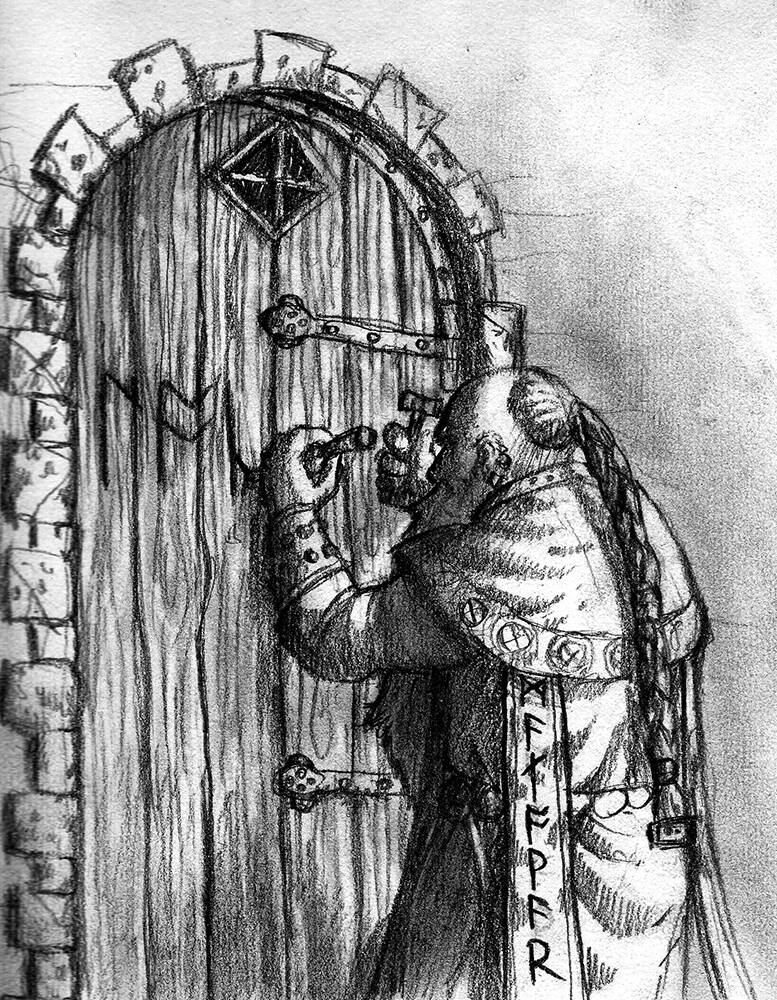
\includegraphics[width=\linewidth]{images/Roch_Hercka/dwarvish_runes.jpg}
	\label{roch:runes}
}{}

However, in return for this deficit, rune casters can learn their craft far more easily.
Each level of a sphere they purchase costs 5 \gls{xp} less than it normally would.
While buying Fate 2 would normally cost 10 for the first level and 15 for the second, rune casters merely need to spend 5 \gls{xp} for the first level and 10 for the second.
If they ever want to use those same sphere through a different path of magic, they must spend 5 \gls{xp} to `repurchase' each level.
For example, someone who could cast both alchemical and runic magic might purchase Conjuration at the second level for a total of 15 \gls{xp}.
They could only use it for runic magics, but later they could spend 5 \gls{xp} to be able to cast the first level with either the alchemy path or the rune casting path.

Runes can never be cast in a subtle way. All castings will be entirely obvious. Ritual castings are a particularly long affair, often taking an entire day's work and always require runes to be dented or impressed into something rather than just written out.

\subsubsection{Mana Stones}
\index{Mana Stones!Runes}

Rune casters mana stones are, of course, runic carvings, and can never be painted onto anything.

\subsection{The Path of Song}

\label{song}\textbf{Spheres}: Aldaron, Enchantment, Fate, Illusion

The character has learnt the magic of song. They can sing illusions into existence, inspire people with great tales and enchant people with a lute. Any instrument, song or performance suffices for casting a spell so long as it is appropriate -- a flute is not usually a good way to magically make people scared.

Song spells appear with a flash of colour -- generally on a cinematically appropriate note. They require some noise to activate so they are difficult to hide, but people will not always make the connection between the start of a spell and the strumming of a lyre.

In order to learn the Path of Song, the mage must have the second level of the Performance Skill. 

\subsubsection{Special Considerations}

Just as with rune magic, song magic can never be cast in an instant.  Their highest level of a sphere can only be cast as a ritual spell, and quick spells are entirely barred, as a song takes time to be invoked with magic.  And as with rune magic, those on this Path need to spend 5 less \gls{xp} each time they buy a level of some magic sphere.

\subsubsection{Mana Stones}
\index{Mana Stones!Song}

The mana stones of the Path of Song are actual songs.
The bard composes a song especially for the purpose; when anyone -- anywhere in the world -- plays the song on the correct instrument the mana can be regained.

If anyone ever pulls mana from the song (either for a spell casting or because they are low on mana) while the song-spell is empty, it is destroyed forever.
The song will be difficult for anyone to remember and will no longer store any mana until someone remakes the spell.

Rare and powerful spell-songs are swapped as currency among bards -- spells which can protect the singer or enchant a crowd.

\end{multicols}

\section[Spellcasting]{Casting Your First Spell}

\begin{multicols}{2}

\subsection{Casting}

Spells are cast by spending a number of \gls{mp} equal to the spell's level, so 1st level spells always cost 1 \gls{mp} and 3rd level spells always cost 3 \gls{mp}.
The character then spends the mana and makes a roll against some \gls{tn} to cast the spell.

\index{Mana}\subsection{Mana}

Anyone can buy some base \gls{mp} which is then modified by their Intelligence.\footnote{See the section on Experience, page \pageref{xp}, for costs of base \gls{mp}.} For example, someone with Intelligence +1 who buys Base \gls{mp} 2 would have a store of 3 \gls{mp} to cast spells. Those with a Base \gls{mp} of 0 can still have some \gls{mp} if their Intelligence Bonus is positive.

If a caster has no \gls{mp} left, they can still cast spells by paying the cost with \gls{hp} instead of \gls{mp}.
The magical energies pull the power they need from the blood and bones of the caster, leaving them with a bleeding nose, raging headache and sometimes stranger effects such as acidic pustules or discoloured skin patches.
Many a desperate caster has died through the use of their own magic rather than an enemy's sword; a wizard with their back to the wall is a dangerous opponent indeed.\iftoggle{verbose}{\footnote{\Glsentrylongpl{hp} cannot be spent instead.}}{}

Mana is a fickle thing -- when lazing \ around a village it can take hours to regain even a little driblet of magic.
When fighting in deep caves, a few minutes' focus can summon most of a mage's magical energies back.
Every scene, characters regenerate 2 Mana plus their Wits Bonus.
If this total would be 0 then the amount of time required to gather a single \gls{mp} increases by 1 scene.
Characters with a Wits score of -2 must wait 2 scenes before regenerating 1 \gls{mp} while those with Wits -3 must wait 3 scenes.

\needspace{15em}
\subsection{Range}

\begin{wrapfigure}{r}{.16\textwidth}

\begin{rollchart}

	Wits & Range \\\hline

	-4 & 1 \\

	-3 & 2 \\

	-2 & 3 \\

	-1 & 4 \\

	0 & 5 \\

	1 & 10 \\

	2 & 15 \\

	3 & 20 \\

	4 & 25 \\

\end{rollchart}

\end{wrapfigure}

Spells have a range of 5 squares plus 5 times the caster's Wits bonus.
A negative Wits Bonus decreases the range by one square per penalty.

\iftoggle{verbose}{
Magic extends all around the character but mages can rarely affect targets anywhere near the range of a good archer.
}{}

Spells which affect a large area are only restricted by where they \emph{start}.
A \textit{Wide Fireball} covering 3 squares might be cast 5 squares away, but it could extend past that, reaching a total of 7 squares.

This range limitation applies to all magic, including Song magic.
While a tune may carry over the hilltops, the force of the magic usually remains close to the caster.

\subsection{Duration}

Some spells are instant -- a ball of fire flashes from the mage and incinerates someone, or a touch grants the favour of the gods, healing FP -- but most are continuous. Continuous spells can be cancelled at will or maintained indefinitely. However, while they are being maintained, the \gls{mp} required to cast them remains spent, lowering the mage's maximum \gls{mp}.

For example, Tauron the elven sorcerer casts a spell on himself to appear as a gnome -- all the better to blend into surrounding society. He spends 1 \gls{mp}. Later, he enchants an animal to be his companion for 2 \gls{mp}. Normally, his maximum \gls{mp} is 6, but he is currently reduced to a maximum of 3 \gls{mp} so long as he continues to be a bear-riding gnome.

These still-active spells are known as \glspl{standingspell}. Some mages operate by continuously casting different spells and then going `empty' when the mana is gone. Others typically operate with \gls{standingspell} alone, casting everything they might need before the day begins and leaving their useful spells `running' but leaving themselves unable to cast more.

\subsection{Spell Types}

Your standard spell takes a while to cast -- normally 1 \gls{round} per level, so a Level 3 spell would normally take 3 \glspl{round} to complete.  Casters can go slower or faster and gain bonuses or penalties to their roll.

\subsubsection{Ritual Spells}

Mages who take their time over spells can attempt a Ritual Spell -- they cast it as a \gls{restingaction}.\footnote{See page \pageref{restingactions}}.
The mage can gain mana slowly, spending some, drawing more from a mana stone or item, then spending more before finally casting the spell.
The mage can gather a number of \gls{mp} equal to double their normal maximum \gls{mp}, ignoring \glspl{standingspell}.
Ritual spells can also be cast as a team effort -- any number of spell casters who are on the same \gls{path} of magic can cast any spell they all know together.
They can each invest \gls{mp} to create \gls{standingspell}, and thereafter any one of them can cancel the spell.

\subsubsection{Quick Spells}

Quick spells can be completed fast enough to cast in combat, costing 3 Initiative points plus the level of the spell.
Such spells always force a little `flash and bang' out as the raw magic hits the air.
Some mages create sparks as they cast spells, others summon dark mists -- it all depends upon the Path of Magic the mage is walking.

Quick Spells are challenging, and require the mage know a spell intimately.  They cannot be cast with the mage's highest spell level.  A mage with Polymorph at level 3 cannot cast level 3 as a Quick Spell.

\subsection{Spell Enhancements}

Spell enhancement increase a spell's level in return for adding some ability.
These enhancements always take the form of adjectives.
For example, the first level \textit{Fireball} spell, has the enhancement ``(1) Enhancement -- Raging'', meaning the mage can cast a \textit{Raging Fireball}, which would count as a second level spell.
The enhancement ``(1) Wide'' can be used on any spell to have it cover a wide area, so while a Fireball spell would normally be level 1, a \textit{Wide, Raging Fireball} would be a level 3 spell.
The spell would then cost 3 \glspl{mp} to cast, and require 6 Initiative Points if cast during combat.

\iftoggle{verbose}{
	\subsection{Spell Failure}
	Spells are always cast, even if the caster does not get the intended result.
	If an illusion spell fails, the illusion persists -- it simply looks obviously magical, like bad CGI.
	If a fireball spell fails, fire still comes, as the mage's mana has to go \emph{somewhere}, even if nothing hits the intended target.
}{}

\end{multicols}

\resumecontents[magic]

\sphere{Metamagic}
\index{Metamagic}

\begin{multicols}{2}

\index{Path Rating}

\noindent
The total \glsentrylongpl{mp} a mage has grants additional spell-casting powers.
The more power a mage has, the more flexible their spells.
A mage with a base mana score of 2 and an Intelligence Bonus of +1 would have a total Metamagic rating of 3.

Every power level offers the caster new spells or -- more often -- enhancements to existing spells.
The enhancements drawn from Metamagic can affect all spells the caster has, not simply the spells listed here.
In this way, spells can be combined for greater effects.

\iftoggle{verbose}{
For example, early invocationists can cast a \textit{Fireball} spell as a Level 1 spell.
With sufficient \glsentrylongpl{mp}, the mage can cast a \textit{Wide Fireball} as a level 2 spell, affecting more targets.
Fireballs can also be enhanced by making them \textit{Raging} when cast at +1 level (which adds +2 to the Damage).
Finally, combining all these effects, a mage could cast a \textit{Wide, Raging Fireball} as a level 3 spell (assuming the mage had level 3 Invocation).
This would inflict $1D6 + 2$ Damage, plus the mage's Intelligence Bonus, over a wide area.
}{}

Anyone who walks any Path of Magic can make use of any of these abilities, even if they haven't bought any spheres.
These spells are not like the formal spells in magical spheres.
They require no words, hand movements, or anything else to use.
However, such spells quickly become expensive.
A level 8 Metamagic spell requires 8 \glspl{mp} to cast, and requires 11 Initiative points.

\spelllevel
\label{detectmagic}

\spell{Identify Item}{Instant}{Academics}{Find out if an item is magical}\\
The mage detects whether or not something is a mana stone (i.e. an item or person which stores mana).

\spelllevel

\spell{Identify Mana}{Instant}{Empathy}{Find out which path of magic made an item}\\
The caster identifies which Path of magic someone is walking, or which Path was used to create an item which holds \glsentrylongpl{mp}.

\spell{Detect Mana}{Instant}{Empathy}{Find out exactly how many \glspl{mp} are in the target}\\
The mage casts the spell on any person or item and finds out how many \glsentrylongpl{mp} the target has, including any mana stones the target has.

\spelllevel

\spell{Imbuing}{Instant}{Empathy}{Add \glspl{mp} to a mana stone}\\
The mage spills any number of mana points into a mana stone created through the same path of magic the mage walks.
If cast as a \textit{Wide} spell, the mage can spend \glspl{mp} to spread between multiple items, but can only Imbue total \glspl{mp} equal to what is spent.

\enhancement{1}{Subtle}{Cast any spell unseen}

Casting an illusion or enchantment on someone with a flashing, loud and generally obvious spell can be quite a give away.
Any caster can attempt to cast a spell while simply whispering and moving their hands slowly and subtly.

People around the mage can still sometimes spot a spell being cast. They use their Wits + Academics in a resisted roll against the mage's Dexterity + Deceit.

\enhancement{1}{Wide}{Widen the spell to hit $Level + Wits$ targets}
The spell extends to cover a wide area -- a total area equal to the spell's level, plus the caster's Wits Bonus.
The squares are always continuous, so a spell targeting four squares could form a $2\times 2$ area, or four continuous squares.

If the spell targets people, one person per square is always a reasonable baseline, but more might be targeted in a narrow tunnel, or fewer if targets are spread out to surround the party.

\spelllevel

\spell{Mana Stones}{Continuous}{Academics}{Create a vessel for \glspl{mp} equal to double the \glspl{mp} you sacrifice}\\
A mana stone is an item which stores mana, and each path of magic has its own version.\footnote{See page \pageref{magic_paths} for more on Paths of Magic.}
Once an item (or creature) is designated as a mana stone, the spell is cast and the mage forfeits any number of \glspl{mp} from their maximum.
For each \gls{mp} forfeited, the mage can store 2 \gls{mp} in the stone.
For example, a mage with 5 \glspl{mp} might pour 3 into a mana stone.
The mage would be left with only 2 \glspl{mp} to use, but the stone would have 6 \glspl{mp}.

Anyone on the same Path of Magic can retrieve the mana from the stone by simply touching it and concentrating.
The spell is always permanent -- no additional mana must be kept aside so that the spell remains active.
Retrieving the mana takes the normal amount of time to use an item -- 8 Initiative points

The mana in mana stones cannot be used to create more mana stones and mages cannot enter their own temporary \gls{mp} into the mana stone.

Mana stones form the basis of all magical items, and \glspl{miracleworker} can only use their traditional mana stones to create magical items.

\subsubsection{Ambient Mana Regeneration}
\label{ambientmana}
\index{Ambient Mana}
These stones always start life empty, but regenerate \glspl{mp} each scene until they reach their maximum.
Mana stones only fill up through the ambient mana in the air.
Typically, this means 2 \glspl{mp} at the end of each scene, or 3 within a deep forest, or anywhere secluded.

However, there is only so much mana to go around.
Multiple mana stones in an area must divide the mana between them.
Whichever has the most empty slots restores mana first, so if one item has 1 out of 5 \glspl{mp} left, while another has 8 out of a maximum 9 \glspl{mp} left, the first item takes ambient \glspl{mp} first, because it has 4 empty points, so it draws more in.
If items are tied, roll a die to see which regenerates \glspl{mp} first.

\iftoggle{verbose}{
	For this reason, adventuring parties cannot make use of dozens of magical items at once.
}{}

\spell{Spell Breaking}{Instant}{Sphere Rating}{Destroy a spell.}\\
The caster can destroy an existing spell, whether that spell is a persistent effect, such as a Polymorph, or a magical item.
The spell requires an opposed roll of Intelligence + the sphere being used.

For example, a priest casts an Aldaron spell.
She has Intelligence +2 and Aldaron 3.
The \gls{tn} is therefore ($7+2+3=$) 12.
Later, an alchemist attempts to dispel the magic.
He rolls with his Intelligence Bonus of +3, but he does not have the Aldaron sphere, so he can add nothing more.
If he fails the roll, he can attempt to try again, turning this into a ritual spell.
However, if that fails, he simply cannot roll again.

\spelllevel

\spell{Pocket Spell}{Instant}{Crafts}{Allow a mana stone to cast a single spell at the cost of 1 permanent \gls{mp} from the mana stone, after which the stone is broken}\\
The pocket spell changes a mana stone so that it can contain one spell.
The mana stone loses access to a single point of mana, and then the mage casts a spell \textit{into} the mana stone.
The pocket spell can then cast the spell once, at which point it ceases to be a mana stone, and all imbued mana returns to the caster.

The mage must cast the spell immediately after \textit{Pocket Spell}, and has no chance to regain mana between castings.

Some mages create scrolls which are destroyed once read.  Some priests of \gls{naturegod} enchant animals with a single spell, just to see how the animal will use it.
The only limitation is that the mana stone must have enough \gls{mp} to cast the spell once.

The pocket spell always produces a single effect.
The mage can create an item which casts an illusion of a dragon, but never a scroll where the user determines the illusion cast.
Any continuous effects last for \arabic{spelllevel} scenes plus the caster's Wits Bonus.

These magical items are activated by a `command word'.
Command words do not necessarily have to be actual words -- they could be entire phrases or gestures.

Pocket spells require the same initiative to use as the spell would require, and use the same Traits as the caster.
For example, if an illusionist made a scroll which created an illusion of a bear, and had Intelligence +2 and Beast Ken +2, the scroll would cast an illusion with a +4 bonus to the roll, no matter who used it.

\spelllevel

\enhancement{1}{Ranged}{Increase any spell's range to line of sight}

Any spell, from any sphere, can be targeted anywhere the mage can clearly sense, breaking all the normal range boundaries of spells.

\spelllevel

\spell{Talisman}{Continuous}{Academics}{Sacrifice one permanent \gls{mp} in a mana stone to let it cast a spell}\\
The mage takes a mana stone and allows it to cast a spell, forging a new magical item. A sword could be made which can summon blinding light, or a ruby could be infused with the power to teleport the caster to a specific nearby location.

Just as with Pocket Spell, above, the mage casts Talisman and the spell to be implanted in succession, while also relinquishing a number of \gls{mp}.
Any number of spells can be cast into the item, so long as each one is implanted within the same casting.

Magical items continue to store \gls{mp} for use by people on that Path of Magic.
However, each spell cast into the item lowers the item's \gls{mp} by one.

Such basic spells always take effect in exactly the same way and use the mage's stats for any rolls. A second level Aldaron spell set to freeze water will always do just that, and can never cast a Sunray. An illusion-generating mask, making the wearer into a bush, will always turn that wearer into a bush, regardless of what the user may want the illusion to be of.

Talismans which do not have enough mana simply fail to cast.
The one exception here is the Path of Song, wherein spell-songs which have too much mana drawn from them simply break, rendering the Talisman-song useless.

\enhancement{2}{Massive}{Increase the target area until it's the size of $level + Wits$ areas}

The spell spreads across a massive space -- indoors this could be multiple rooms, outdoors it could be a field, or a massive segment of a forest.
Massive spells target a number of areas equal to the spell's level plus the caster's Wits.
\iftoggle{verbose}{%
This spell has the usual range, so if a caster cannot also cast at long-range, the spell must begin in the area the caster currently stands.
}{}

\spelllevel

\enhancement{Varies}{Combined}{Add a second spell effect to the target}

A secondary spell can be combined to throw at the same target.
The combined spells have a single target.
Any applicable enhancements, such as \textit{Wide}, affect both spells.

The smaller spell adds a number of levels equal to half its own level.

For example, a priest of \gls{wargod} might cast a \textit{Raging Fireball} at someone, alongside \textit{Curse}.
The highest level spell there is \textit{Raging Fireball} at level 2, and the other is at level 1 and only costs half the usual \glspl{mp}.
With the two spells together, the total cost is 3 \glspl{mp}, and the spell takes 7 Initiative points to cast.
The caster has an Intelligence score of +3, so the target is hit with $2D6+1$ damage from the fireball, and loses $1D6+2$ \glspl{hp} directly.

\enhancement{1}{Sentient}{Allow the spell to make its own decisions}

The mage can make any spell gain some measure of sentience.
Typically, this is made to allow magical items to activate upon a condition, such as a door which turns from solid stone back to wood once the password is stated.
Such spells can also select their own targets, such as acid which can hit a specific person in the dark, or around a corner.
A conjuration spell could be cast over a massive area, but only turn particular areas of water into ice, or a \textit{Fireball} spell could target only a caster's enemies.

The item acts upon its own Initiative score, and uses the mage's Wits score as its Initiative Factor.
Sentient illusions can converse on their own, with simple-minded and predictable (but plausible) personalities.
Sentience levitating swords can fight on their own, without aid.

Sentient spells have about the same ability to perceive the environment as the caster would were they present.
Such spells could also use other spells to find out further information, such as a swords which detects someone's Code, and then activates other abilities selectively.

Sentient spells only create one sentience per spell, even with \textit{Wide} spells.
A spell which levitates 4 daggers would only be able to use one at a time, and an illusion of a banquet hall, full of dancers, would only have enough focus to make them all dance, but could not make each one individually speak.

Sentient spells have the same Code as their caster, so a caster who followed \gls{justicegod} and then cast an enchantment on an animal would create a very law-abiding animal, while an alchemist who followed the Code of Experience would cast very inquisitive illusions, that persistently tried new things.

\spelllevel

\spell{Artefact}{Instant}{Academics}{As `Talisman', but the item gains a full sphere of magic}\\
This functions just like the Talisman spell, except that the mage can imbue a full sphere's level.
If the item has Necromancy level 2, the item can cast any Necromancy spell of level 2 or less.
If it has Invocation level 3, it can cast any spell at level 3 or less.
Each sphere (but not each level) reduces the item's \gls{mp} by 1, just as with \textit{Pocket Spell}.
The item's user simply focusses on what they want, and the spell casts.

\iftoggle{verbose}{
Once the spell Artefact spell is cast, the spell's level must be cast into it as part of the same spell.
Therefore, a mage creating an item with the 3rd level of Necromancy must first spend \arabic{spelllevel} \glspl{mp}, followed by 3 \glspl{mp} to place the necromancy sphere into the item.
}{}


\spelllevel

\spell{Greater Mana Stone}{Continuous}{Academics}{Allow a mana stone to store 3 \glspl{mp} per point sacrificed}\\
This spell works like a standard mana stone, except stones cast with this enhancement store 3 \gls{mp} per point sacrificed instead of 2.
So a \gls{miracleworker} sacrificing 4 \glspl{mp} would create a mana stone capable of storing 12 \glspl{mp}.

\stopcontents[magic]

\end{multicols}

